% Compile: pdflatex main && bibtex main && pdflatex main && pdflatex main
\documentclass[11pt]{article}

\usepackage[margin=1in]{geometry}
\usepackage{amsmath,amssymb,amsfonts}
\usepackage{booktabs}
\usepackage{graphicx}
\usepackage{hyperref}
\usepackage{microtype}
\usepackage{natbib}

\title{Shared Structure Without Stronger Scale Dependence:\\
Qualifying the Platonic Scaling Prediction in Cross-Modal Astronomy}
\author{Anonymous authors}
\date{}

\begin{document}
\maketitle

\begin{abstract}
The Platonic Representation Hypothesis predicts increasing representational convergence with model scale~\citep{huh2024platonic}.
We ask whether that relationship becomes clearer when cross-modal correspondence is measured through substantially different probes on matched Legacy Survey--HSC embeddings~\citep{duraphe2025platonicuniverse}.
Shared sparse representations raise held-out neighbourhood correspondence substantially above the dense baseline, but the additional alignment they recover is approximately independent of model size.
Within-family probe\(\times\)scale interactions are correspondingly small and mixed in sign (SAE mean \(D{=}{-}5.2{\times}10^{-4}\); BSF mean \(D{\approx}0\); \(6/11\) positive in each case).
A nonlinear alignment trained without paired objects~\citep{jha2025vec2vec} also recovers nontrivial relational geometry, yet its size dependence is non-monotonic.
The resulting picture is simple: probe choice strongly affects how much shared structure is visible, but much less clearly affects how that structure changes with raw model size.
This suggests that parameter count alone is unlikely to be the full control variable for representational convergence.
\end{abstract}

\section{Introduction}
\label{sec:intro}

Representations from independently trained models often become more aligned as capability and scale increase~\citep{huh2024platonic}.
The Platonic Representation Hypothesis (PRH) interprets this as convergence toward a shared statistical model of reality~\citep{huh2024platonic}.
In astronomy, matched survey embeddings provide a particularly direct test: previous work reports increasing mutual \(k\)-nearest-neighbour (mKNN) alignment with model capacity~\citep{duraphe2025platonicuniverse}.

A basic ambiguity remains.
Measured alignment depends on how the representation is read.
If a structured probe exposes substantially more Legacy\(\leftrightarrow\)HSC correspondence than dense embeddings, does that extra correspondence appear preferentially in larger models?

We test that question directly.
On a matched held-out evaluation, shared-basis sparse autoencoders (SAEs)~\citep{gao2025sae,lan2024saeuniversality} and block-sparse featurizers (BSFs)~\citep{fel2026bsf} increase neighbourhood overlap across every model-size rung.
We define the resulting lift as
\[
L_R(P)=M_R(P)-M_{\mathrm{dense}}(P),
\]
and ask whether \(L_R(P)\) itself grows with \(P\).
It does not.
The corresponding within-family interaction,
\[
D_R=\Delta M_R-\Delta M_{\mathrm{dense}},
\]
is small and mixed in sign.

We then use a qualitatively different probe, an unpaired nonlinear alignment inspired by \citet{jha2025vec2vec}.
It recovers nontrivial relational structure without paired training objects, but again shows no clean monotonic relationship with model size.

The central result is therefore not that any particular probe ``fails to scale.''
It is that changing the probe changes the \emph{level} of measured correspondence much more reliably than it changes the \emph{size response}.

\section{Experimental setup and alignment probes}
\label{sec:setup}

\subsection{Legacy\(\leftrightarrow\)HSC model-size ladders}

We use the official UniverseTBD Legacy Survey~\citep{dey2019legacy}\(\leftrightarrow\)HSC~\citep{miyazaki2018hsc} matched embeddings~\citep{duraphe2025platonicuniverse}.
Each rung pairs the same architecture size across surveys (\(n{=}16{,}384\)).
The model families are AstroPTv2 (15, 95, 850M)~\citep{smith2024astropt},
ConvNeXtv2 (nano--large)~\citep{woo2023convnextv2},
DINOv2 (small--giant)~\citep{oquab2024dinov2},
ViT (base--huge)~\citep{dosovitskiy2021vit},
and I-JEPA (huge, giant)~\citep{assran2023ijepa}.
The unpaired analysis covers ConvNeXt and DINOv2.

\subsection{mKNN and matched evaluation}

For paired representations \(A\) and \(B\),
\[
M_k=\frac{1}{n}\sum_i
\frac{\lvert \mathcal N_k^A(i)\cap \mathcal N_k^B(i)\rvert}{k},
\]
using cosine neighbours with self-exclusion~\citep{huh2024platonic,duraphe2025platonicuniverse}.
Neighbour lists are sliced to \(k\) before intersection.
Our primary scale is \(k{=}10\).
Under a uniform-neighbour null, the expected overlap is \(k/(n{-}1)\)~\citep{groger2026aristotelian}.

The original full-catalog dense score is retained only to connect to the scaling analysis of \citet{duraphe2025platonicuniverse}.
All probe\(\times\)scale comparisons use the same held-out query IDs, full gallery, \(k\), self-exclusion, and object set (\(n_{\mathrm{test}}{=}3277\)).
Dense, SAE, and BSF are therefore directly comparable in both level and size response.

\subsection{Dense, SAE, and BSF probes}

The dense probe uses the raw \(\ell_2\)-normalised embeddings with cosine mKNN.

For SAE, we encode both surveys with pretrained TopK sparse autoencoders~\citep{gao2025sae}, then fit a Ridge map from Legacy codes into the HSC basis using train IDs only, with train-only IDF weighting (\texttt{shared\_side1\_basis\_idf}).
The mapping direction is fixed in advance.
Dictionary width \(F{=}2048\) and seed \(0\) are shared across the ladder; TopK sparsity varies with the available checkpoint (\(k\in\{18,\ldots,23\}\)).

For BSF, we replace SAE codes with Vanilla BSF full signed codes~\citep{fel2026bsf} (\(G{\approx}512\) blocks) and apply the same shared-basis protocol.

For each within-family adjacent step \(P_j\to P_{j+1}\), we compute
\[
D_{R,j}
=
\Delta M_{R,j}
-
\Delta M_{\mathrm{dense},j}
=
L_R(P_{j+1})-L_R(P_j),
\]
for \(R\in\{\mathrm{SAE},\mathrm{BSF}\}\).
This is the quantity of interest: whether the extra correspondence exposed by the structured probe itself increases with size.

\subsection{Unpaired relational probe}

Our second analysis uses a DualEncoder inspired by \citet{jha2025vec2vec}.
Each survey is mapped through a model-specific MLP into a shared latent \(Z{=}256\) and decoded back.
Training combines reconstruction, RBF-MMD, cycle consistency, and Gram-matrix geometry preservation with equal weights (80 epochs, hidden width 512, two seeds).
The two training sets are disjoint (\(5500\) objects per survey), so the model never sees paired cross-survey correspondences.

Evaluation uses a held-out paired set (\(n{=}2884\)) and measures neighbourhood agreement between the translated representation and the true opposite-survey embedding.
This is a different relational functional from the matched SAE/BSF comparison, so we use it to test the \emph{shape} of size dependence rather than to rank absolute mKNN values across methods.

\section{Results}
\label{sec:results}

\subsection{Structured probes reveal substantially more correspondence}
\label{sec:level}

Against the matched held-out dense baseline at \(k{=}10\), SAE lifts every rung (mean \(+0.0056\), range \(+0.0025\)--+0.0127), while BSF produces a larger mean lift of \(+0.0076\) (range \(+0.0017\)--+0.0168).
For example, ConvNeXt nano moves from \(0.0092\) dense to \(0.0149\) with SAE and \(0.0161\) with BSF; I-JEPA giant moves from \(0.0176\) to \(0.0274\) and \(0.0321\), respectively.
The dense paper-style scores themselves are already above chance (\(\approx0.007\)--\(0.018\), mean \(0.0115\)), but the structured probes expose substantially more correspondence.

Figure~\ref{fig:multiples} shows the main visual pattern: large vertical shifts between probes, with much smaller changes in the shape of the within-family trajectories.

\begin{figure}[t]
\centering
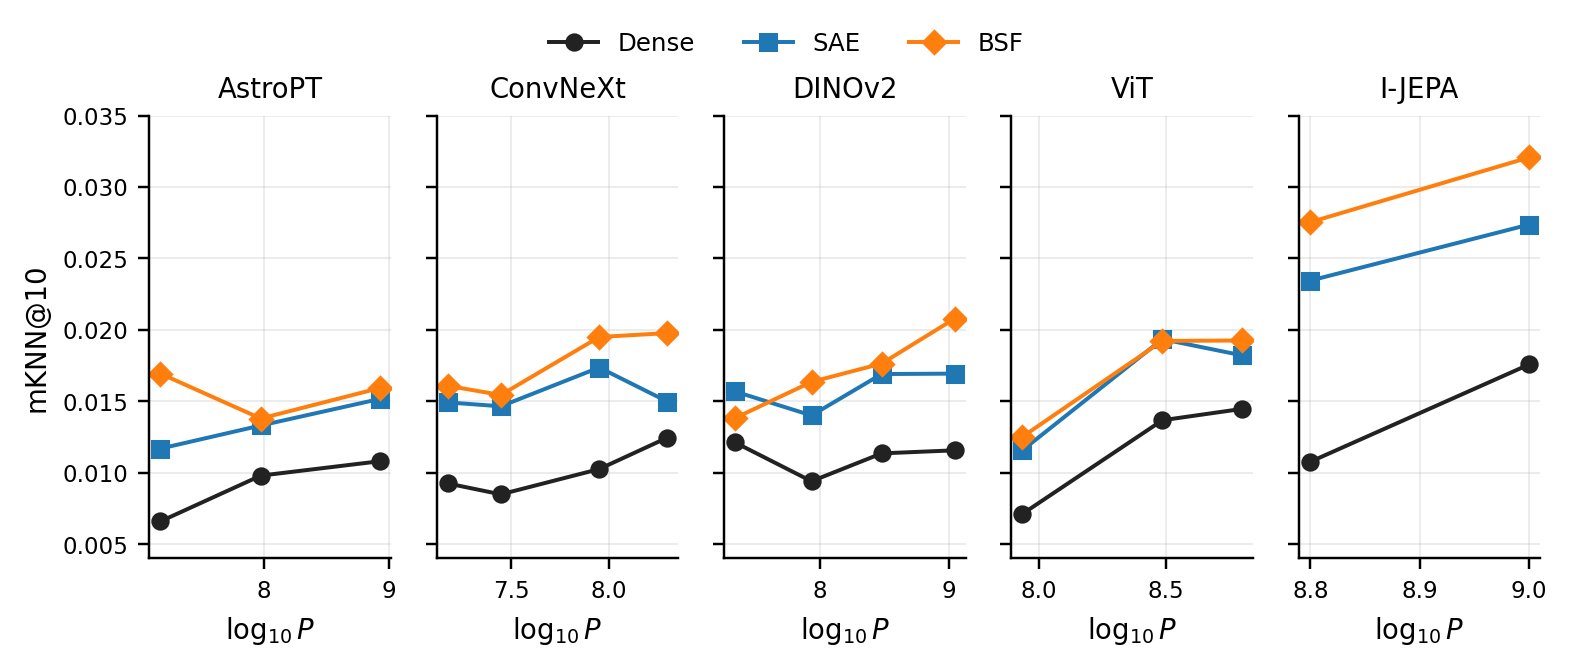
\includegraphics[width=\linewidth]{figures/legacy_small_multiples_k10.png}
\caption{Held-out mKNN@10 across Legacy\(\leftrightarrow\)HSC model ladders using identical queries and galleries for dense, shared SAE, and shared BSF.
Probe choice changes the level of measured correspondence substantially more than the within-family size trajectory.}
\label{fig:multiples}
\end{figure}

\subsection{The extra correspondence does not strengthen systematically with scale}
\label{sec:interact}

Under the original paper-style dense evaluation, \(8/11\) adjacent size steps are positive (one-sided \(p{=}0.113\)), reproducing the mild direction of the earlier astronomy scaling result on this Legacy-only subset.
The main analysis, however, is the matched held-out comparison.

The 11 within-family probe\(\times\)scale interactions cluster around zero (Figure~\ref{fig:interact}b).
For SAE, mean \(D{=}{-}5.2{\times}10^{-4}\), median \(+4.9{\times}10^{-4}\), range \([-4.6,+1.2]{\times}10^{-3}\), with \(6\) positive and \(5\) negative.
For BSF, mean \(D{\approx}0\), median \(+1.2{\times}10^{-4}\), range \([-6.3,+5.2]{\times}10^{-3}\), again with \(6\) positive and \(5\) negative.
The sign test is correspondingly uninformative (\(p{=}1\)).
Mean absolute interactions (\(|D_{\mathrm{SAE}}|{=}0.0015\), \(|D_{\mathrm{BSF}}|{=}0.0022\)) are no larger than the typical dense adjacent step (\(|\Delta M_{\mathrm{dense}}|{=}0.0025\)).

The same result appears in the lift itself.
Spearman correlation between \(L_R(P)\) and \(\log_{10}P\) is \(+0.11\) for SAE and \(+0.13\) for BSF.
In other words, the structured probes expose more shared structure, but that extra structure does not preferentially emerge in the larger models.

Raw adjacent-sign counts are consistent with this reading rather than being the main result.
On the matched holdout they are \(9/11\) for dense, \(7/11\) for SAE, and \(9/11\) for BSF.
BSF can rise with size while its \emph{increment over dense} remains approximately size-independent.

\begin{figure}[t]
\centering
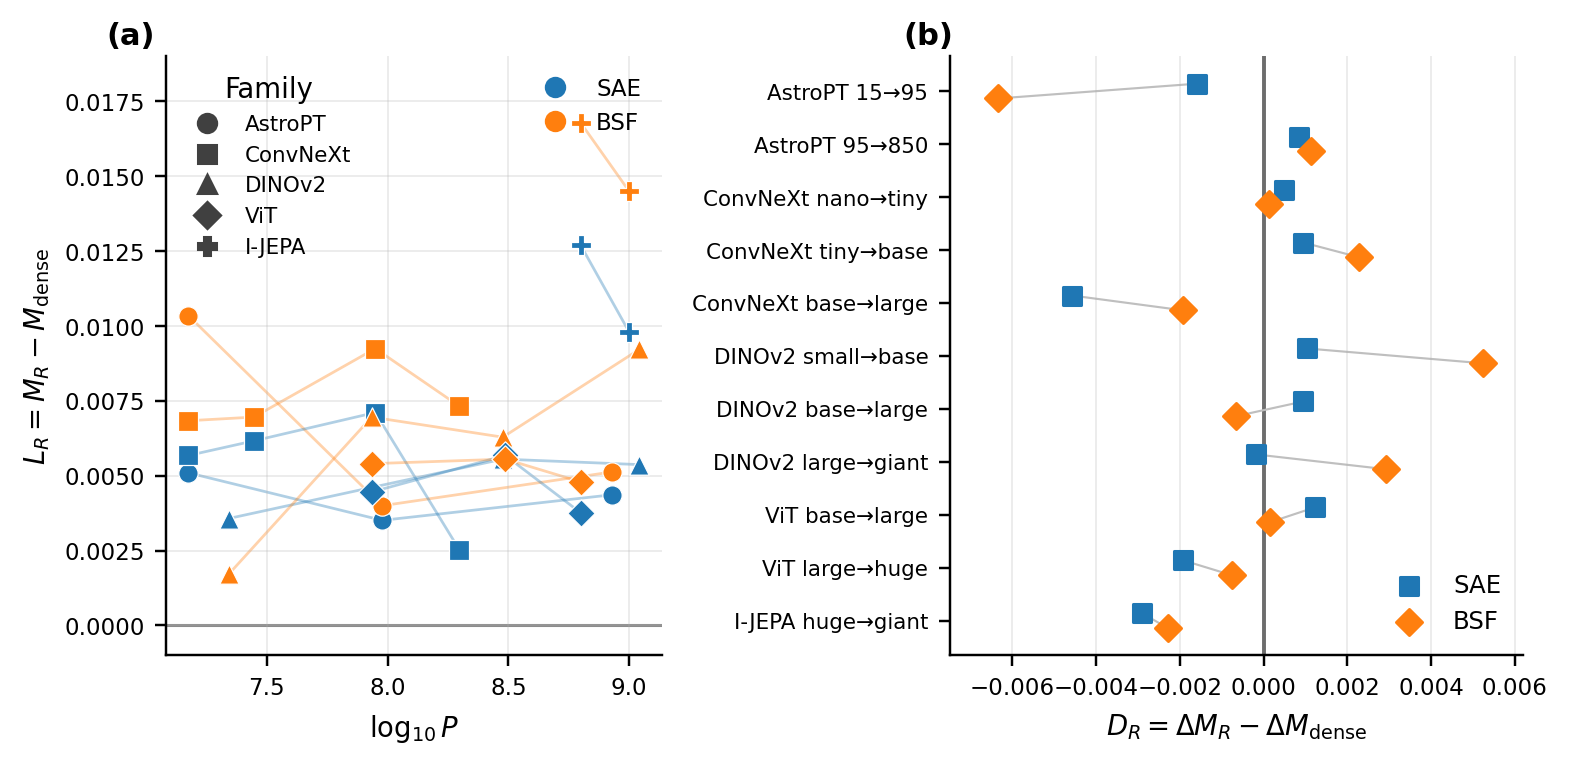
\includegraphics[width=\linewidth]{figures/probe_scale_interaction.png}
\caption{(a)~Matched held-out lift \(L_R(P)\) versus \(\log_{10}P\).
(b)~Adjacent probe\(\times\)scale interaction \(D_R=\Delta M_R-\Delta M_{\mathrm{dense}}\) for the same 11 within-family steps.
The lift is positive across the ladder, while its change with model size remains small and mixed in sign.}
\label{fig:interact}
\end{figure}

\subsection{Unpaired alignment gives the same qualitative size picture}
\label{sec:unpaired}

The unpaired probe recovers nontrivial relational structure, but its model-size trajectories are again non-monotonic.
For ConvNeXt, mKNN@10 follows
\[
0.016\to0.012\to0.023\to0.012,
\]
while DINOv2 gives
\[
0.022\to0.019\to0.020\to0.019.
\]
Only \(2/6\) adjacent steps are positive.
With six transitions, the trajectory itself is more informative than a significance test.

This does not put unpaired alignment on the same absolute scale as SAE or BSF.
Its value here is that a substantially different relational probe does not reveal the clean monotonic size dependence that the dense-coordinate explanation would predict.

\begin{figure}[t]
\centering
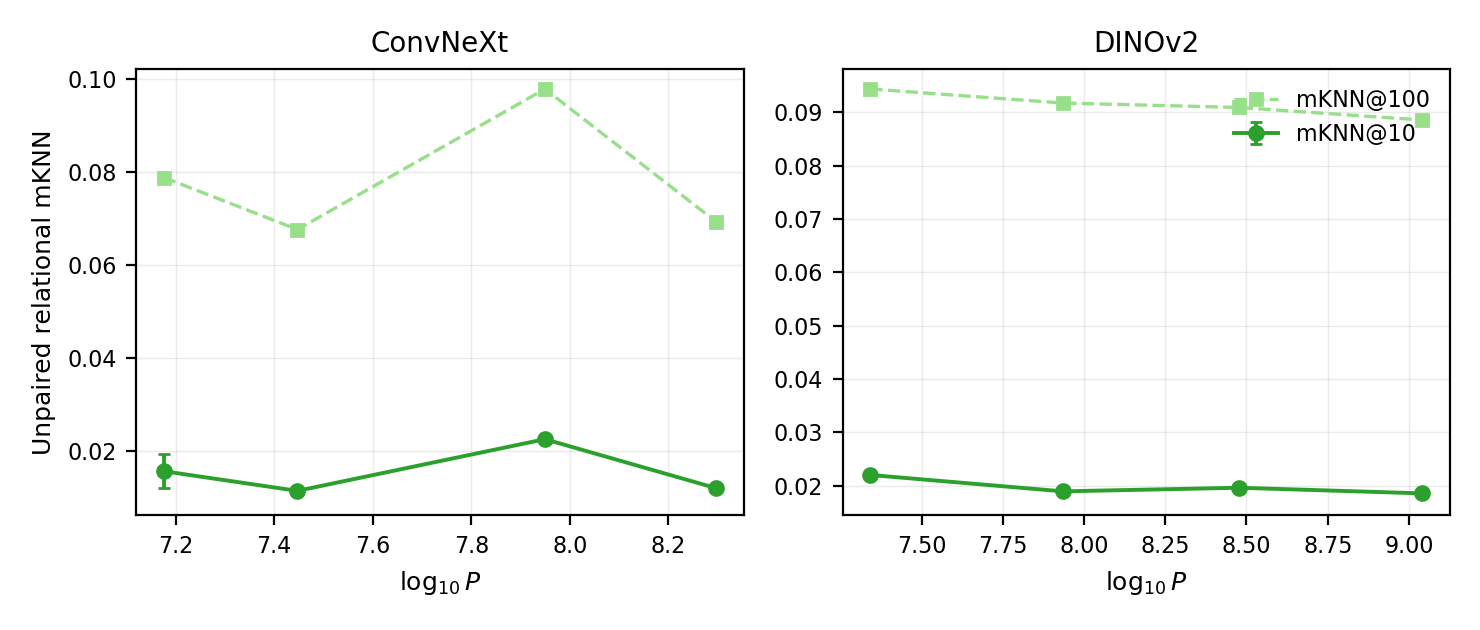
\includegraphics[width=0.82\linewidth]{figures/unpaired_legacy_mknn_vs_size.png}
\caption{Unpaired DualEncoder relational mKNN versus \(\log_{10}P\) (mean \(\pm\) seed sd; two seeds).
Solid: mKNN@10. Dashed: mKNN@100.
The curves are non-monotonic across both available families.}
\label{fig:unpaired}
\end{figure}

\section{Discussion and limitations}
\label{sec:disc}

The main result is a separation between alignment magnitude and scale dependence.
SAE and BSF expose substantially more Legacy\(\leftrightarrow\)HSC correspondence than dense embeddings, yet the corresponding probe\(\times\)scale interactions remain small and heterogeneous.
The unpaired result points in the same direction from a different construction.
Taken together, this makes it difficult to explain the weak size response simply as a consequence of having chosen the wrong representation.

One possibility is that raw parameter count is simply not the right variable.
It is not an invariant measure of functional complexity: parameters can be added redundantly without materially changing the represented function.
Model size may therefore stand in for a more relevant quantity, such as the pressure to achieve capability under constrained computational resources.
Under that view, representational convergence could depend more directly on efficiency or compression pressure than on parameter count itself.
We treat this as a hypothesis for future work.
The connection to computationally relative notions of structure such as epiplexity~\citep{finzi2026epiplexity} is suggestive, but not required for the present result.

The main limitations are straightforward.
There are only 11 paired adjacent transitions, and the unpaired analysis covers two families.
SAE TopK sparsity is not perfectly homogeneous across the ladder (\(k\in\{18,\ldots,23\}\), with fixed \(F\) and seed).
The unpaired analysis uses a different training and evaluation construction by design.
Finally, learned alignment procedures can induce correspondence in ways that an analytical mKNN chance baseline does not capture; pipeline-refit permutation nulls are therefore a natural next control~\citep{groger2026aristotelian}.

\section{Conclusion}
\label{sec:conc}

Structured probes substantially increase measured cross-modal correspondence, but the additional correspondence they expose does not systematically increase with model size.
A qualitatively different unpaired relational probe gives the same broad picture over the available ladders.
Probe choice strongly affects how much shared structure is visible; its interaction with raw model scale is considerably weaker and less consistent.

This suggests that the next question is not simply whether larger models become more Platonic, but what quantity actually governs representational convergence.

\section*{Acknowledgments}
Code and exact configurations will be released with the camera-ready version.

\bibliographystyle{plainnat}
\bibliography{references}

\end{document}
